\chapter{Método de pesquisa}
\label{cap:metodologia}

Neste capítulo descreveremos os métodos de pesquisa que serão utilizados. Inicialmente, haverá uma breve  introdução a respeito do modelo de estimação da dívida técnica proposto seguido por uma explicação a respeito de como iremos avaliá-lo usando um estudo de caso  quantitativo.

\section{Introdução}

Nesta pesquisa proporemos um modelo para a estimação dos juros da dívida técnica em projetos de desenvolvimento de software. Nesse modelo, consideramos os juros como a variação negativa, na produtividade do projeto, causada pela existência da dívida técnica. Conforme ilustrado na Figura \ref{fig:cap_metodo_niveis_abstracao}, esse modelo possui dois níveis de abstração. O primeiro é conceitual e baseia-se em uma definição abstrata tanto da produtividade de um projeto quanto do principal da dívida técnica. No segundo nível, já há uma definição das métricas que serão utilizadas para a estimação dos juros em projetos reais. O segundo nível de abstração é na verdade uma instância do modelo de primeiro nível. Futuramente podem ser definidas diversas instâncias do modelo de primeiro nível, cada uma terá de ser criada de acordo com as características dos projetos que serão avaliados. Por exemplo, em uma situação onde deseja-se estimar os juros da dívida técnica de um projeto web provavelmente serão utilizadas métricas de produtividade diferentes das métricas de um projeto de software. No Capítulo \ref{estimacao:juros} forneceremos  uma definição precisa a respeito do modelo de estimação dos juros e seus níveis de abstração. 

Para avaliarmos a aplicabilidade tanto do modelo de primeiro nível quanto de segundo nível, realizaremos um estudo de caso quantitativo e exploratório utilizando dados de 1.870 projetos hospedados publicamente na plataforma GitHub. O objetivo dessa avaliação é verificar,  por meio de métodos estatísticos,  os resultados da aplicação do modelo nesses 1.870. Os seguintes itens serão avaliados:

\begin{itemize}
\item Existência de uma correlação entre a quantidade de dívida técnica de um projeto e a sua produtividade.  A existência dessa correlação é uma evidência de que seja viável a estimação dos juros da dívida técnica por meio de modelos baseados em métricas de produtividade. 
\item Existência de uma consistência no modelo específico criado para estimar a dívida técnica de projetos de software livre. Ou seja, vamos avaliar a aplicação de uma instância do modelo de estimação. Essa instância foi criada observando as particularidades dos projetos de software livre e também observando as limitação nos dados que temos disponíveis da plataforma GitHub.
\end{itemize} 



  \begin{figure}[H]
  \centering
  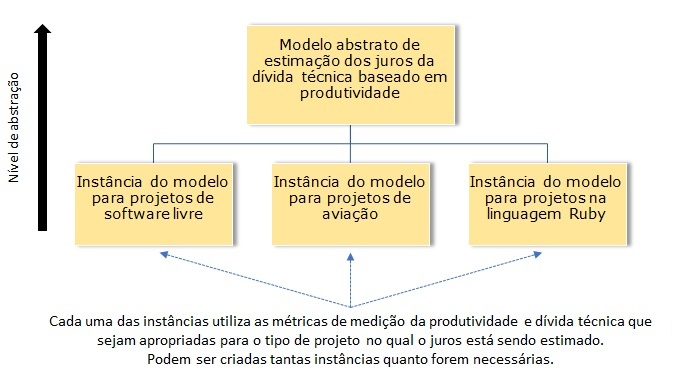
\includegraphics{capitulo_metodo/NiveisDeAbstracoesModelo.jpg} 
  \caption{Níveis de abstração do modelo de estimação dos juros da dívida técnica. }
  \label{fig:cap_metodo_niveis_abstracao} 
\end{figure}




\section{Pesquisa quantitativa}




De acordo com Creswell\cite{w2016research}, uma pesquisa quantitativa tem como foco principal a quantificação de relacionamentos ou a comparação de um ou mais grupos. Adicionalmente, conforme explicado por Wohlin et al.\cite{wohlin2003empirical}, as pesquisas quantitativas são apropriadas quando existe a necessidade de testar o efeito de alguma atividade ou manipulação. Segundo Wang at al. \cite{wang201331}, a abordagem quantitativa disponibiliza uma série de ferramentas para descobrir, com um determinado nível de confiança, a verdade a respeito de um objeto de estudo. O que difere substancialmente uma pesquisa quantitativa de outra qualitativa é seu grau de  objetividade a respeito dos fenômenos avaliados. Na abordagem quantitativa há pouco ou nenhuma margem para que haja, durante o processo de coleta de dados, uma interpretação dos indivíduos relacionados com o evento analisado. Ao invés disso, são utilizados apenas fatos que não dependem de sensações, reflexões, intuições ou qualquer outra forma subjetiva de avaliação. Isso faz com que os dados numéricos sejam predominantes em pesquisas quantitativas.  Essa característica permite que, utilizando poucos recursos, um grande volume de dados possa ser coletados e analisado.  Amaratunga et al. \cite{amaratunga2002quantitative} lista algumas das principais características de uma pesquisa quantitativa:

\begin{itemize}
\item Permitem a replicação e a comparação de resultados.
\item Independência entre o observador e o objeto observado.
\item A confiabilidade e validade dos resultados podem ser determinadas de forma mais objetiva.
\item Enfatiza a necessidade de formular hipóteses para subsequentes verificações.
\end{itemize}

São muitas as atividades necessárias para a realização de uma pesquisa quantitativa. Essas atividades podem ser dívidas em duas fases. A primeira fase é constituídas por atividades de planejamento, obtenção e validação dos dados necessários para a avaliação do objeto da pesquisa. Esses dados podem ser obtidos de diversas formas. As mais comuns são a realização de questionário, experimentos, estudos de caso e, mais recentemente, a mineração de repositórios. A segunda fase consiste na avaliação desses dados utilizando métodos matemáticos, estatísticos ou computacionais.  

Conforme argumentado por Brown, N et al.\cite{brown2010managing}, há uma predominância na utilização de métodos qualitativos nas pesquisas a respeito da dívida técnica e isso pode levar a conclusões baseadas em intuições atraentes, porém não necessariamente corretas. Essas conclusões incorretas podem ser explicadas pela existência de dados obtidos por meio de declarações imprecisas. Essas declarações podem ser dadas pela dificuldade que as pessoas envolvidas com os projetos de software têm em assumir suas deficiências ou falhas. Por isso, Brown, N et al.\cite{brown2010managing} indica a necessidade da criação de modelos baseados em abordagens quantitativas para viabilizar a criação de rigorosas técnicas de gerenciamento da dívida técnica que possam ser aplicadas em projetos de larga escala. Neste trabalho iremos propor um modelo para estimação da dívida técnica. Para analisarmos a validade desse modelo, iremos realizar um estudo de caso quantitativo utilizando dados de projetos de software hospedados na plataforma GitHub. 

\subsection{Mineração de repositórios}

Plataformas como GitHub, SourceForge e Bitbucket ganharam popularidade devido à evolução nas ferramentas de controle de versão e o reconhecimento, por parte da comunidade de software,  das vantagens de utilizar ferramentas de colaboração. Além de ferramentas para armazenamento e organização do código, essas plataformas fornecem uma variedade de facilidades para a interação entre os colaboradores dos projetos. Com isso, essas ferramentas acumularam uma quantidade imensa de dados sobre os projetos hospedados e a forma como colaboradores interagem com esses projetos. Esses dados têm sido reconhecidos como altamente relevantes para as pesquisas quantitativas na área de engenharia de software. Foi chamado de mineração de repositórios de software \cite{bai2008mining} o conjunto de técnicas de investigação que utilizam informações provenientes de repositórios de software. Como exemplos de estudos que exploram essas técnicas, podemos citar aqueles envolvendo a predição de defeitos \cite{wang2014software}, propagação de mudanças \cite{wiese2015predicting} e confiabilidade do software \cite{de2015software}. Neste trabalho, utilizaremos a mineração de repositórios de software para extrairmos os dados para o estudo de caso. 

\section{O estudo de caso}

 De acordo com Wohlin et al.\cite{wohlin2003empirical}, um estudo de caso é um método de pesquisa onde são utilizados dados de situações reais. Diferentemente de um experimento, no estudo de caso o pesquisador tem menos ou nenhum controle sobre os acontecimentos.  No contexto de projetos de software, um estudo de caso tem como objetivo monitorar as atividades realizadas durante o projeto. Segundo Yin, Robert K\cite{yin2011applications}, existem dois tipos de estudo de caso: os únicos e os múltiplos. Os estudos de casos únicos são aqueles onde os dados são obtidos de um único ``caso'',  que pode ser um projeto, uma empresa, um indivíduo ou qualquer outra unidade que seja apropriada para o estudo do objeto da pesquisa. Por outro lado, um estudo de caso múltiplo envolve diferente unidades de interesse. Ou seja, são consideras diversas empresas, projetos, indivíduos e etc. A realização de caso múltiplos é mais indicada já que os mesmos ela facilita generalização dos resultados obtidos por fornecerem múltiplas visões a respeito do objeto de pesquisa. Tendo isso em vista,  para avaliarmos o modelo de estimação do comportamento dos juros da dívida técnica descrito no capítulo \ref{estimacao:juros}, realizaremos um estudo de caso múltiplo envolvendo milhares de projetos armazenados em um repositório de software.

\subsection{Etapas do estudo de caso}



 O estudo de caso será realizado em 5 etapas conforme resumido na  Figura \ref{fig:cap_metodo_resumo_etapas}.  Foi desenvolvida  uma ferramenta para automatizar grande parte das atividades realizadas em cada etapa. Mais detalhe sobre a ferramenta de apoio serão fornecidos na seção \ref{cap_estudo_caso_ferramenta}. A seguir forneceremos uma descrição panorâmica a respeito de cada uma das etapas do estudo de caso. Uma descrição detalhada de cada uma das etapas será fornecida no Capítulo \cite{cap_estudo_caso}.
 
\label{sec:Passos_Elaboracao_Modelo}

  \begin{figure}[H]
  \centering
  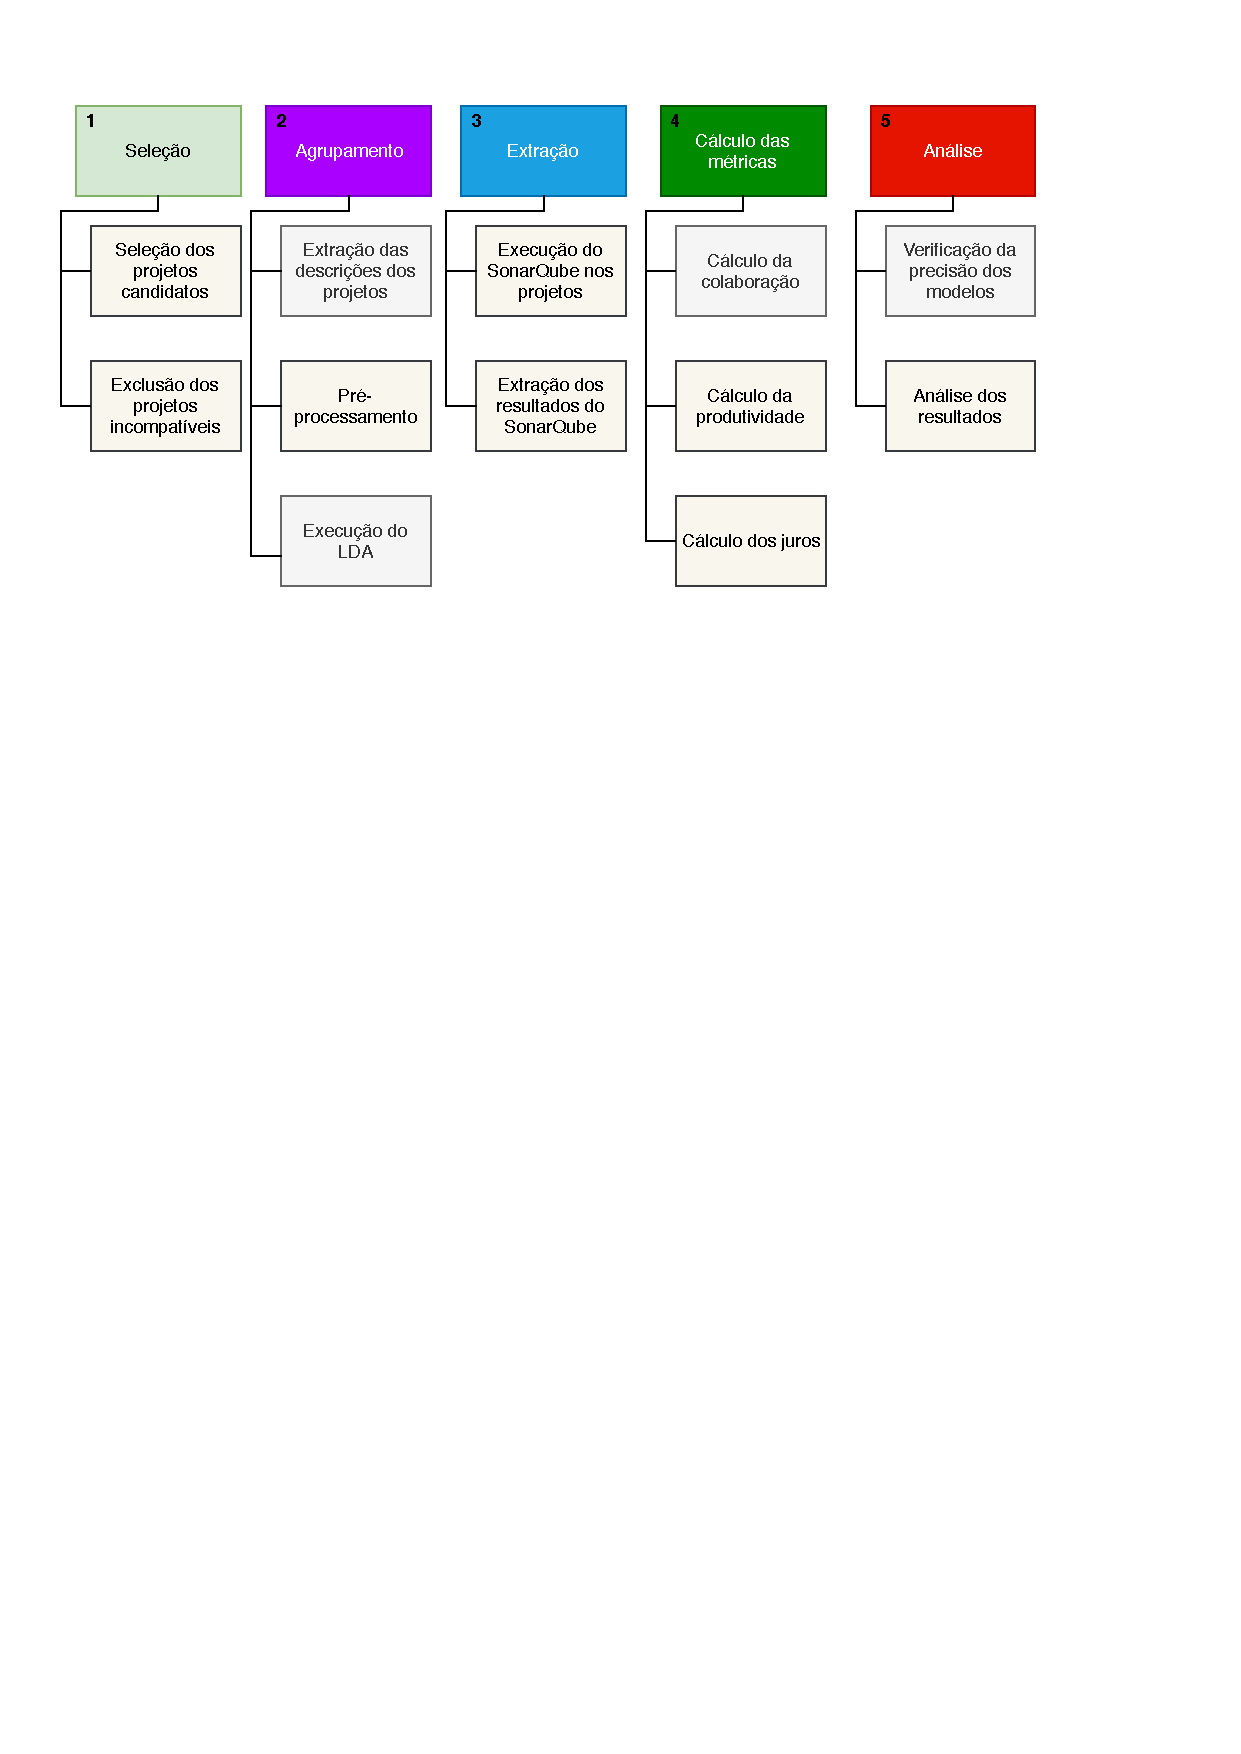
\includegraphics{capitulo_metodo/ResumoEtapas.pdf} 
  \caption{Resumo das etapas do estudo de caso. }
  \label{fig:cap_metodo_resumo_etapas} 
\end{figure}

\subsubsection{Etapa 1 - Seleção dos projetos} 


Foram usados diversos critérios para selecionar os projetos incluídos no estudo de caso. Os primeiros deles estão relacionados com a necessidade de verificar se um repositório presente no GitHub realmente se trata de um projeto de software. Isso é necessário já que por disponibilizar a possibilidade de gratuitamente armazenar arquivos, muitas vezes o GitHub é utilizado para armazenar conteúdo que não é um projeto de software. É comum encontrar arquivos de sites, exercícios escolares, contratos e diversos outros itens que não têm relação com o objeto desta pesquisa. Na literatura, são encontradas pesquisas que fornecem heurísticas para identificar se um repositório no GitHub é um projeto de software ou não. Um exemplo é  o trabalho de Kalliamvakou et. al.\cite{kalliamvakou2014promises} onde são elencados diversos perigos encontrados na mineração de dados no GitHub. Outro trabalho relevante é o de Russel. M.\cite{russell2013mining} onde o autor faz um análise abrangente a respeito da mineração de dados no GitHub como também em diversas outras plataformas. A seleção dos projetos foi realizada utilizando uma combinação dessas heurísticas juntamente com outras regras apropriadas para este estudo. Algumas das regras utilizadas foram:

\begin{itemize}
\item Projetos realizados na linguagem Java. Essa regra foi definida por dois motivos. O primeiro motivo é a diferença que existe entre as dívidas técnicas de uma linguagem e outras. Por exemplo, existem dívidas específicas para linguagens orientadas a objetos que não são possível de serem encontradas em linguagens procedurais. O segundo motivo é técnico e está relacionado com as limitações da ferramenta utilizada para a extração de métricas. Ela possui uma maior compatibilidade com a linguagem Java.
\item Projetos no qual a documentação estive escrita em inglês. O motivo dessa restrição foi a necessidade de separar os projetos por domínio de aplicação. Essa separação foi feita aplicando técnicas de machine learning  na documentação dos projetos.  A inclusão de múltiplas linguagens iria trazer uma complexidade substancial a esse processo. Além disso, a técnica de classificação utilizada não era compatível com textos em múltiplas linguagens.
\end{itemize}


\subsubsection{Etapa 2 - Agrupamentos dos projetos semelhantes}


De acordo com Kitchenham et. al.\cite{kitchenham2004software}, a comparação de produtividade entre projetos de software deve ser feita considerando o domínio de cada um deles. Ou seja, não faz sentido comparar a produtividade de um projeto da área da aviação, que possui padrões extremamente rígidos de qualidade, com um projeto de uma aplicação para a internet. Por isso, os projetos utilizados no estudo de caso foram divididos em domínios de aplicação como sistemas gerenciadores de banco de dados, jogos, frameworks, linguagens de programação e etc.

Inicialmente foram consideradas algumas estratégias para estimação do domíno do projeto. Uma delas foi a proposta de Idri. et. al.\cite{idri2001fuzzy}. Nela, os autores utilizam um modelo baseado em lógica Fuzzy para estimar o domínio de um projeto de software. Além disso, foram estudas outras abordagens baseadas no código fonte da aplicação. Entre elas estão o trabalho de Yamamoto et. al.\cite{yamamoto2005measuring} e a ferramenta MudaBlue, proposta por Kawaguchi et. al.\cite{kawaguchi2006mudablue}. Essas abordagens não foram utilizadas já que dependiam de informações que não tínhamos acesso ou da construção do projeto. Como utilizamos uma abordagem automática, muitas vezes não era possível compilar os projetos devido a algum erro no código, incompatibilidade com o ambiente ou falta de alguma dependência. 

Para estimar o domínio de cada projeto, utilizamos uma estratégia baseada em \textit{Latent Dirichlet allocation} (LDA)\cite{blei2003latent,hoffman2010online,blei2002latent}. O LDA é uma técnica de aprendizado de máquina que basicamente consegue classificar documentos em assuntos. Essa técnica foi aplicada na documentação dos projetos a fim de agrupá-los de acordo com o domínio estimado e comparar a produtividade apenas entre projetos de um mesmo domínio.




\subsubsection{Etapa 3 - Extração dos dados}


Foi utilizada a ferramenta SonarQube\cite{campbell2013sonarqube} para realizar a extração das métricas dos projetos. Os dados obtidos podem ser divididos dois grupos de métricas: um geral com informações diversas a respeito do projeto e o outro com as informações a respeito da dívida técnica. Todas as métricas foram obtidas observando a evolução temporal dos projetos. Isso foi feito ordenando as atualizações nos códigos fonte de forma sequencial e as dividindo em 5 pontos. Então as métricas foram obtidas para cada um desses pontos. Isso foi feito para viabilizar a análise temporal da evolução da dívida técnica do projeto e melhorar as estimativas. Essa estratégia foi necessária porque a dívida técnica de um projeto pode variar muito com o tempo. Um projeto pode começar com muita dívida e depois realizar fatorações para diminuí-la substancialmente. Ao extrairmos as métricas em diferentes momentos da evolução do software, estamos considerando essa variação temporál.


\subsubsection{Etapa 4 - Cálculo das métricas de produtividade}

Nessa etapa os dados obtidos dos projetos foram usados para calcular as métricas de produtividade do projeto. O cálculo de alguns dos componentes desses métricas de produtividade foi feito utilizando uma versão adaptada do algoritmo PageRank\cite{page1999pagerank}. Nesta versão, a qualidade das contribuições dos colaboradores foi medida usando, entre outros fatores, dados a respeito da popularidade do colaborador. Isso envolveu medir a reputação de cada colaborador que contribuiu com o projeto. Como são milhares de projetos e colaboradores, houve uma alta complexidade em criar algoritmos que pudessem realizar esses cálculos em um tempo viável. Por isso, esse cálculo das métricas de produtividade foi separado em uma etapa exclusiva ao invés de considerado como um passo auxiliar da extração de dados.


\subsubsection{Etapa 5 -Análise dos resultados}


Nesta etapa, análisamos estatísticamente todos os dados obtidos nas etapas anteriores. Para tal, utilizaremos técnicas da estatística inferencial e métodos da inteligência artificial. Os objetivos nessa etapa é avaliar a aplicabilidade do modelo de estimação dos juros da dívida técnica em projetos reais.  









 










